
\documentclass[11pt,a4paper,openany]{report}
\usepackage[T1]{fontenc}
\usepackage[utf8]{inputenc}
\usepackage{lmodern}
\usepackage{microtype}
\usepackage{amsmath,amssymb,amsthm,mathtools,bm}
\usepackage{booktabs,array,longtable,tabularx}
\usepackage{xcolor}
\usepackage[margin=22mm,headheight=23pt]{geometry}
\usepackage{enumitem}
\usepackage{fancyhdr}
\usepackage{fancyvrb}
\usepackage{graphicx}
\usepackage{url}
\usepackage{xurl}
\usepackage{hyperref}
\definecolor{finblue}{HTML}{1F5A99}
\definecolor{fingreen}{HTML}{19733A}
\definecolor{finorange}{HTML}{D55E00}
\definecolor{finred}{HTML}{A61B1B}
\definecolor{finviolet}{HTML}{6A3D9A}
\definecolor{fingray}{HTML}{4D4D4D}

\hypersetup{
  unicode=true,
  colorlinks=true,
  linkcolor=finblue,
  citecolor=fingreen,
  urlcolor=finblue,
  pdftitle={FIN Current State after Programs P267--P280},
  pdfauthor={Krzysztof Żuchowski},
  pdfsubject={Spectral identifiability, operational instruments, falsification boundaries, and the conditional passage from information to physics},
  pdfkeywords={FIN, spectral operator, Stieltjes measure, Schur complement, quantum instrument, current tomography, renormalization, Landauer principle, operational physics}
}
\pagestyle{fancy}
\fancyhf{}
\fancyhead[L]{\small FIN Programs P267--P280}
\fancyhead[R]{\small Release 10.25}
\fancyfoot[C]{\thepage}

\setlength{\parindent}{0pt}
\setlength{\parskip}{0.55em}
\setlist{nosep,leftmargin=2em}
\setcounter{tocdepth}{2}
\setcounter{secnumdepth}{3}
\emergencystretch=3em
\newcommand{\one}{\bm 1}
\newcommand{\C}{\mathbb C}
\newcommand{\R}{\mathbb R}
\newcommand{\Z}{\mathbb Z}
\newcommand{\statusProven}{\textcolor{fingreen}{[Proven]}}
\newcommand{\statusStrong}{\textcolor{finblue}{[Strong evidence]}}
\newcommand{\statusModerate}{\textcolor{finviolet}{[Moderate evidence]}}
\newcommand{\statusWeak}{\textcolor{fingray}{[Weak evidence]}}
\newcommand{\statusSpeculative}{\textcolor{finorange}{[Speculative]}}
\newcommand{\statusRefuted}{\textcolor{finred}{[Refuted]}}

\begin{document}
\hypersetup{pageanchor=false}
\begin{titlepage}
\centering
\vspace*{8mm}
{\Large\bfseries FIN --- Release 10.25\par}
\vspace{10mm}
{\Huge\bfseries Current State of the Theory\par}
\vspace{4mm}
{\LARGE\bfseries after Research Programs P267--P280\par}
\vspace{7mm}
{\Large Spectral identifiability, operational instruments,\\
falsification boundaries, and the conditional passage\\
from information to physics\par}
\vspace{15mm}
{\Large Krzysztof \.Zuchowski\par}
\vspace{2mm}
{\normalsize Independent Researcher --- Fractal Information Theory Project\par}
\vspace{2mm}
{\normalsize ORCID:
\href{https://orcid.org/0009-0002-0909-3613}{0009-0002-0909-3613}\par}
\vspace{8mm}
{\large 28 July 2026\par}
{\normalsize Publication --- Preprint; Version 1.0.0\par}
\vfill
\begin{minipage}{0.91\textwidth}
\small
\textbf{Central conclusion.}
FIN has a rigorous finite spectral-operator core, exact context memory, and
constructible operational interfaces. It does not yet internally generate a
physical unit, an orientation choice, a laboratory instrument, or a unique
physical interpretation.

\medskip
\textbf{Minimal surviving architecture.}
\[
(A,\mathcal C)
\quad\longrightarrow\quad
(A,\mathcal C,\mathfrak O)
\quad\longrightarrow\quad
(A,\mathcal C,\mathfrak O,\mathfrak C,\mathfrak S).
\]
The last arrow remains conditional on operational, conversion, and
symmetry-breaking resources.

\medskip
\textbf{Repository.}
\url{https://github.com/hyconiek/Fractal-Nadsoliton-Theory}

\textbf{License.} CC BY 4.0.
\end{minipage}
\vfill
\end{titlepage}
\hypersetup{pageanchor=true}
\pagenumbering{roman}
\chapter*{Publication statement}
\addcontentsline{toc}{chapter}{Publication statement}
This monograph reports all executed Programs P267--P280, integrates their
results with the current FIN state map, states the mathematical and physical
boundaries explicitly, and recommends Programs P281--P294. Synthetic audits
are never described as laboratory evidence. The strict and legacy kernels
remain separated, QW-2191 remains open, and no physical-role or Theory of
Everything closure is claimed.

\tableofcontents
\clearpage
\pagenumbering{arabic}

\chapter*{Confidence convention}
\addcontentsline{toc}{chapter}{Confidence convention}

\begin{itemize}
\item 
\textbf{\statusProven{}} --- an exact finite-dimensional theorem, analytic identity, or exhaustive result in the explicitly declared class. Numerical computation may be used as a reproducible certificate.

\item 
\textbf{\statusStrong{}} --- a deterministic, preregistered-style synthetic audit with frozen data generation, controls, metrics, and thresholds.

\item 
\textbf{\statusModerate{}} --- a stable conclusion in a declared model class that still depends on an additional equivalence, source, or interpretation.

\item 
\textbf{\statusSpeculative{}} --- a proposed object or research direction not yet supported by a sufficient theorem or test.

\item 
\textbf{\statusRefuted{}} --- an explicit counterexample or no-go theorem in the stated class.

\end{itemize}

Mathematical status is not physical status. In particular, \textbf{\statusProven{}} means that a mathematical statement follows under its written hypotheses. It does not mean that nature realizes the hypotheses.

\chapter{Executive summary}

All fourteen Programs P267--P280 were executed. They extend the earlier operator-memory analysis without reopening the repository's closed selector, generic bridge, role-transfer, or field-equation lanes.

The present scientific conclusion is:

\begin{quote}\itshape
\textbf{FIN currently has a rigorous finite operator core, a rigorous context-dependent memory calculus, and several constructible operational layers. It does not yet possess an internal theorem that generates a physical unit, an orientation choice, a laboratory instrument, or a unique physical interpretation.}

\end{quote}

The strongest new positive and negative results are:

\begin{enumerate}
\item 
The finite visible pole-residue measure of a Stieltjes self-energy is unique. Nevertheless, its numerical inverse is severely ill-conditioned: uniqueness does not imply stable recovery. \textbf{\statusProven{}} for uniqueness; \textbf{\statusStrong{}} for the frozen noisy inversion audit.

\item 
Schur reduction has an executable categorical core: identity, associative composition, and preservation of the positive cone were verified over 50,000 nested chains with maximum residual \(8.88\times10^{-16}\). This is not yet machine-checked proof-assistant formalization and is not a sheaf or contextuality theorem. \textbf{\statusProven{}}

\item 
The five independent FIN current observables admit one informationally minimal six-outcome POVM. The response has rank five and condition number one on the nontrivial response subspace. The construction proves mathematical measurability, not apparatus realizability. \textbf{\statusProven{}}

\item 
Every linear isometric lifting of a reduced \(n<12\) Laplacian has rank at most \(n-1\), whereas the connected strict generator has rank eleven. Therefore zero-padding, replication, or any equivalent rank-preserving linear lift cannot restore the strict operator. A genuine size-restoring RG object must inject complement dynamics or compare only an explicitly defined observable quotient. \textbf{\statusProven{}}

\item 
A quantum instrument supports an exact process-information ledger:

\[
   D(\rho\Vert\sigma)
   \ge
   D(p\Vert q)
   +
   \sum_y p_yD(\rho_y\Vert\sigma_y).
   \]

The remainder is information discarded by the instrument channel. This bridge is conditional because the instrument, state space, and quantum postulates are supplied rather than derived from FIN. \textbf{\statusProven{}}

\item 
The one permitted legacy-completion atom

\[
   A_{\rm legacy}^{(+)}
   =
   A_{\rm legacy}
   +
   \gamma\!\left(I-\frac{\mathbf1\mathbf1^\top}{12}\right)
   \]

repairs positivity at \(\gamma=7.7101445453\), but fails to reproduce the strict spectral fingerprint or self-energy. It is therefore a cone repair, not a legacy-to-strict completion theorem. \textbf{\statusProven{}}

\item 
No production P241 laboratory bundle is present. Only schemas and empty headers exist. The confirmatory P242 pipeline is therefore not authorized. Software can check custody metadata; it cannot manufacture independent evidence. \textbf{[Executed no-admission certificate]}

\item 
A two-flux finite-difference design exhibits the expected noise-bias optimum at \(h=0.1118278\) in the frozen synthetic model. The median relative error is \(1.15\%\), but the noise model is not yet a detector likelihood. \textbf{\statusStrong{}}

\item 
Four hundred frozen positive-circulant nulls all remain outside the strict spectral-fingerprint tolerance. A deterministic perturbation theorem gives a certified exclusion radius for every null. This is not a distribution-free false-positive probability. \textbf{\statusProven{}}

\item 
Two calibrated time slices obey an exact necessary-and-sufficient test for a homogeneous symmetric semigroup. Static dynamics and uniform rescaling pass; shape drift and mixture memory fail. Without an independent clock, generator scale and elapsed time remain exactly degenerate. \textbf{\statusProven{}}

\item 
Controlled interventions make a two-parameter adaptive law identifiable inside a frozen finite candidate family. They do not derive the law from the strict kernel or exclude laws outside the panel. \textbf{\statusProven{}} within the panel; \textbf{\statusStrong{}} for the synthetic selection.

\item 
A nonlinear reservoir benchmark finds one task-specific FIN advantage: the FIN reservoir exceeds all sixty matched controls on NARMA10, but not on delay, nonlinear prediction, or parity. This does not establish a general computational or biological advantage. \textbf{\statusStrong{}}

\item 
Shannon or quantum relative information becomes free energy only after a Hamiltonian \(H\), a temperature \(T\), and Boltzmann's constant \(k_B\) are supplied:

\[
    D(\rho\Vert\gamma)
    =
    \beta\bigl(F(\rho)-F(\gamma)\bigr),
    \qquad
    \gamma=\frac{e^{-\beta H}}{Z}.
    \]

The identity is exact, but it proves that the dimensional bridge is conditioned on conversion data rather than generated by dimensionless information alone. \textbf{\statusProven{}}

\item 
Scale and orientation form an independent product torsor \(\mathbb R_{>0}\times\mathbb Z_2\). An operational section \(s=(\kappa,\varepsilon)\) supplies both a dimensional scale and an orientation, but positive rescaling cannot choose orientation and orientation reversal cannot choose scale. The construction organizes the missing resources; it does not generate them. \textbf{\statusProven{}}

\end{enumerate}

\begin{figure}[htbp]
\centering
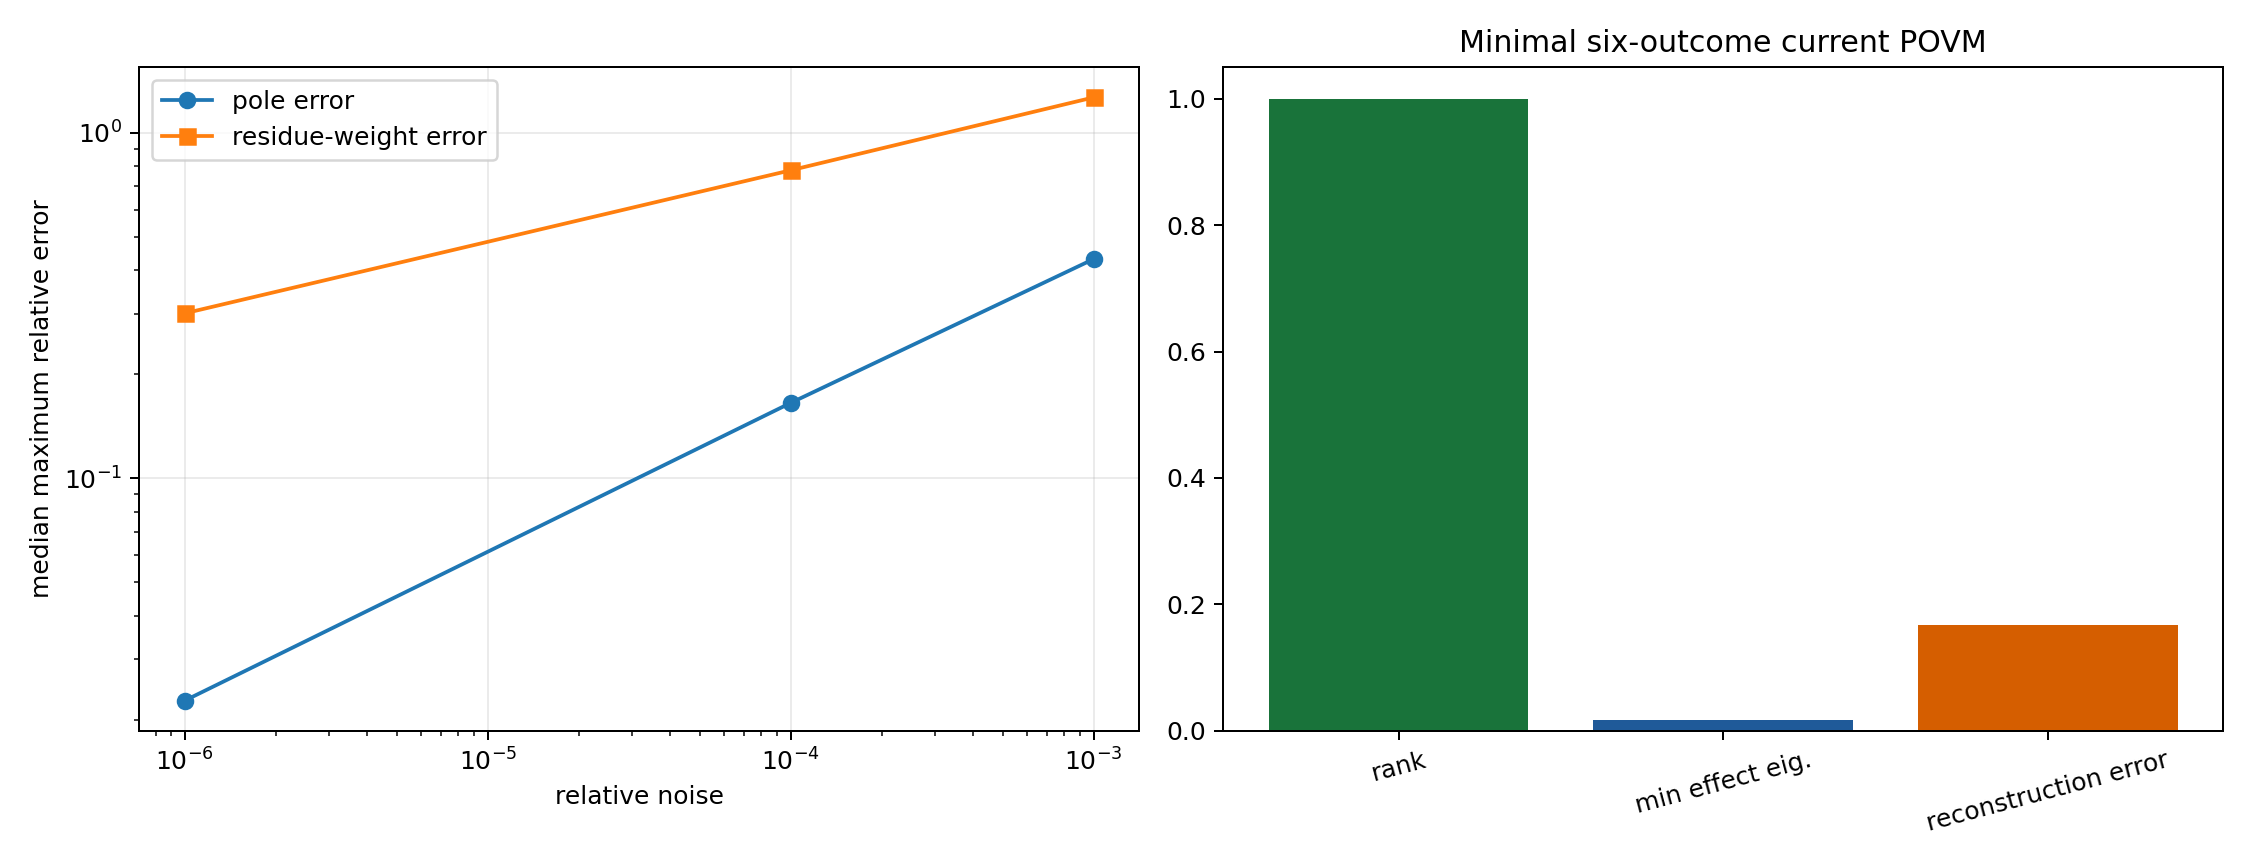
\includegraphics[width=0.97\textwidth]{FIN_Programs_267_280_Figures/p267_p269_measure_povm.png}
\caption{Visible Stieltjes atoms, the severe noise sensitivity of inverse recovery, and the six-outcome current POVM.}
\end{figure}

\chapter{Scope, ontology, and non-negotiable separations}

\section{Ontological statement used by the project}

The repository's internal ontology treats the nadsoliton as primordial fractal information in a solitonic state:

\[
\text{nadsoliton}
\longrightarrow
\text{light}
\longrightarrow
\text{matter}
\longrightarrow
\text{emergent observer}.
\]

No informational substrate below the nadsoliton is introduced in this report. This ontology is recorded as the project's intended interpretation. It is not used as a premise in the finite operator proofs.

\section{Kernel split}

Two kernels must remain distinct:

\[
K_{\rm legacy,ont}(d)
=
\alpha_{\rm geo}
\frac{\cos(\omega d+\phi)}
{1+\beta_{\rm tors}d},
\]

up to the precise repository convention for placement of the amplitude, and

\[
K_{\rm strict,gate}(d)
=
\frac{\cos(\omega d+\phi)}
{1+\beta d^\eta}.
\]

The legacy kernel is an intermediate bridge object. The strict kernel is the later enriched working object and contains nonlinear compression/\allowbreak{}damping and certified phase/\allowbreak{}topological structure not present in legacy. This report does not silently substitute one for the other.

No legacy physical-role formula is transferred to strict. In particular, relations involving \(\alpha_{\rm geo}\), \(\beta_{\rm tors}\), electroweak parameters, electromagnetic couplings, or gravity hierarchies remain outside the conclusions unless a separate bridge and role-transfer theorem is provided.

\section{Strict selector obstruction}

The strict-core uniqueness obstruction QW-2191 remains open. Earlier directional and chiral constructions may receive or transport an orientation, but no current result supplies a unique, non-premise internal sign. P280 packages the missing scale and orientation resources; it does not close them.

\section{What this report does not claim}

This report does not claim:

\begin{itemize}
\item 
a Theory of Everything;

\item 
a Standard Model or general-relativistic derivation;

\item 
a role-bearing total Lagrangian \(L_{\rm total}\);

\item 
a completed legacy-to-strict bridge;

\item 
a strict physical length, time, mass, energy, or action scale;

\item 
a derived Born rule or physical measurement instrument;

\item 
laboratory confirmation;

\item 
Lorentz invariance, locality, continuum field theory, particle content, or experimentally identified couplings.

\end{itemize}

\chapter{Minimal current mathematical architecture}

The present structure is most economically represented by four layers.

\section{Spectral generator}

Let \(V=Z_{12}\), let \(d(x,y)\) be cyclic distance, and define

\[
W_{xy}=K_{\rm strict}(d(x,y)),\qquad x\ne y.
\]

The frozen strict profile used in P267--P280 is

\[
K_{\rm strict}(d)
=
\frac{\cos(0.18575\,d+0.16250)}
{1+d^{1.8}},
\qquad d=1,\ldots,6.
\]

The conservative generator is

\[
A=\operatorname{diag}(W\mathbf1)-W.
\]

It satisfies

\[
A=A^\ast,\qquad A\mathbf1=0,\qquad A\succeq0,
\]

and therefore generates two mathematically valid time families:

\[
U_t=e^{-itA},\qquad P_t=e^{-tA}.
\]

\(U_t\) is unitary wave evolution. \(P_t\) is a positive contraction and, for a graph Laplacian, a Markov/\allowbreak{}diffusive semigroup. The same spectrum controls both. This duality is mathematical; deciding which channel an experiment implements requires a physical preparation, clock, coupling, environment, and readout.

\section{Context and memory}

For an accessible context \(E\subset V\), with hidden complement \(H\), write

\[
A=
\begin{pmatrix}
A_{EE} & A_{EH}\\
A_{HE} & A_{HH}
\end{pmatrix}.
\]

The frequency-domain reduced generator is

\[
A_E^{\rm eff}(z)
=
A_{EE}
-
\Sigma_E(z),
\qquad
\Sigma_E(z)
=
A_{EH}(zI+A_{HH})^{-1}A_{HE}.
\]

Because \(A_{HH}\succ0\) for a proper hidden block of a connected Laplacian,

\[
\Sigma_E(z)
=
\int_{(0,\infty)}
\frac{d\mathsf M_E(\mu)}{z+\mu},
\qquad
d\mathsf M_E(\mu)\succeq0.
\]

This positive operator-valued measure is the most durable mathematical interpretation of FIN's context memory. It unifies resolvent reduction, Green response, hidden-state memory, and completely monotone relaxation without requiring a microscopic physical story.

\section{Operational object}

The operator alone is not an experiment. A minimally specified operational model requires

\[
\mathfrak O
=
(\mathcal S,\mathcal P,\mathcal T,\mathcal I,
\mathcal E,\mathcal M,\mathcal R),
\]

where:

\begin{itemize}
\item 
\(\mathcal S\) is a state space;

\item 
\(\mathcal P\) is a family of preparations;

\item 
\(\mathcal T\) is a calibrated time or control parameter;

\item 
\(\mathcal I\) is an instrument;

\item 
\(\mathcal E\) is an environment or channel model;

\item 
\(\mathcal M\) is an apparatus/\allowbreak{}POVM model;

\item 
\(\mathcal R\) is an event-level record and custody protocol.

\end{itemize}

P269 constructs one mathematical \(\mathcal M\) for currents. P271 supplies one conditional \(\mathcal I\). P273 audits \(\mathcal R\) and finds that the external record is absent. These constructions show that the operational layer can be specified, not that the strict kernel uniquely generates it.

\section{Physicalization resources}

The smallest current physicalization package has at least two independent resource classes:

\[
\mathfrak P
=
\mathfrak O
\oplus
\mathfrak C
\oplus
\mathfrak S,
\]

where

\[
\mathfrak C=(H,T,k_B,\kappa_t,\kappa_\ell,\ldots)
\]

contains conversion/\allowbreak{}calibration resources and

\[
\mathfrak S=(\varepsilon,\text{orientation source/coupling})
\]

contains a sign or symmetry-breaking resource. P279 and P280 prove that conditional bridges exist once these resources are supplied. They do not prove that \(\mathfrak C\) or \(\mathfrak S\) emerges from the strict spectral object.

\chapter{Results matrix}

\begin{center}
\begingroup\small
\setlength{\tabcolsep}{2.5pt}
\renewcommand{\arraystretch}{1.16}
\begin{longtable}{@{}p{0.085\textwidth}p{0.356\textwidth}p{0.180\textwidth}p{0.239\textwidth}@{}}
\toprule
\textbf{Program} & \textbf{Principal result} & \textbf{Status} & \textbf{Boundary} \\
\midrule
\endhead
P267 & unique visible Stieltjes pole-residue measure; unstable inverse & \statusProven{} /\allowbreak{} \statusStrong{} & invisible modes and global stability remain open \\
P268 & executable category core for Schur reductions & \statusProven{} & not proof-assistant formalization; no sheaf theorem \\
P269 & minimal six-outcome POVM for five currents & \statusProven{} /\allowbreak{} \statusStrong{} & apparatus calibration remains external \\
P270 & rank-defect no-go for linear isometric RG lifting & \statusProven{} & nonlinear/\allowbreak{}complement or quotient comparison remains possible \\
P271 & quantum process-information ledger & \statusProven{}, conditional & instrument and quantum structure supplied \\
P272 & positive-shift legacy cone repair fails strict match & \statusProven{} & only one completion atom tested \\
P273 & no admissible external P241 evidence & Executed no-admission certificate & P242 remains unauthorized \\
P274 & optimal synthetic two-flux separation & \statusStrong{} & no detector-level likelihood \\
P275 & certified fingerprint exclusion radii & \statusProven{} & finite frozen null set only \\
P276 & calibrated two-time semigroup theorem & \statusProven{} & rejects homogeneity but does not identify cause \\
P277 & intervention identifies one adaptive law in finite panel & \statusProven{} /\allowbreak{} \statusStrong{} & no strict source law \\
P278 & one task-specific nonlinear reservoir advantage & \statusStrong{} & no general computational advantage \\
P279 & exact information-to-free-energy conversion identity & \statusProven{}, conditional & \(H,T,k_B\) are supplied axioms \\
P280 & scale-orientation product torsor and conditional section & \statusProven{}, conditional & neither resource is internally generated \\
\bottomrule
\end{longtable}
\endgroup
\end{center}

\chapter{P267 --- Identifiability and stability of the visible Stieltjes measure}

\section{Visible measure}

For the frozen context, the trace response is

\[
s(z)=\operatorname{tr}\Sigma_E(z)
=
\sum_{j=1}^{r}\frac{w_j}{z+\mu_j},
\qquad
\mu_j>0,\quad w_j>0.
\]

The three visible poles and trace weights are:

\begin{center}
\begingroup\small
\setlength{\tabcolsep}{2.5pt}
\renewcommand{\arraystretch}{1.16}
\begin{longtable}{@{}p{0.148\textwidth}p{0.356\textwidth}p{0.356\textwidth}@{}}
\toprule
\textbf{\(j\)} & \textbf{\(\mu_j\)} & \textbf{\(w_j\)} \\
\midrule
\endhead
1 & 1.1710910206 & 1.3714541785 \\
2 & 1.5263637131 & 1.1927171397 \\
3 & 1.8883091819 & 0.1937651612 \\
\bottomrule
\end{longtable}
\endgroup
\end{center}

The minimum pole separation is \(0.3552726926\).

\section{Uniqueness theorem}

\textbf{Theorem P267.} Let

\[
s(z)=\sum_{j=1}^{r}\frac{w_j}{z+\mu_j}
\]

be a finite positive atomic Stieltjes transform with distinct \(\mu_j>0\) and nonzero \(w_j\). Exact knowledge of \(s\) on any open real interval determines the visible pole-residue measure uniquely.

\textbf{Proof.} If two such representations agree on an open interval, the identity theorem makes their rational continuations identical. Their pole sets therefore agree. Equality of the principal part at each pole gives the corresponding residue. \(\square\)

For the operator-valued response, the same argument applies entry by entry and recovers each nonzero positive residue matrix.

\section{Stability falsification}

Forty fits were run at each relative-noise level on 48 logarithmically spaced points \(z\in[0.03,8]\).

\begin{center}
\begingroup\fontsize{7}{8.4}\selectfont
\setlength{\tabcolsep}{2.5pt}
\renewcommand{\arraystretch}{1.16}
\begin{longtable}{@{}p{0.155\textwidth}p{0.150\textwidth}p{0.199\textwidth}p{0.154\textwidth}p{0.203\textwidth}@{}}
\toprule
\textbf{Relative noise} & \textbf{Median maximum pole error} & \textbf{95\% pole error} & \textbf{Median maximum weight error} & \textbf{95\% weight error} \\
\midrule
\endhead
\(10^{-6}\) & 0.0228 & 0.1315 & 0.3005 & 0.7358 \\
\(10^{-4}\) & 0.1654 & 7.2928 & 0.7794 & 4.4354 \\
\(10^{-3}\) & 0.4314 & \(1.95\times10^5\) & 1.2668 & \(4.58\times10^3\) \\
\bottomrule
\end{longtable}
\endgroup
\end{center}

The extreme upper tails are optimizer excursions produced by an ill-conditioned rational inverse, not evidence of new modes. They falsify any claim that analytic uniqueness automatically gives a robust reconstruction algorithm.

\textbf{Verdict.} The visible measure is uniquely identifiable in exact arithmetic, but stable recovery requires regularization, pole-count control, uncertainty quantification, and experimental design. Decoupled or zero-residue hidden modes remain unidentifiable in principle.

\chapter{P268 --- Executable Schur category core}

Let the objects be nonempty contexts \(E\subseteq V\). For \(E\subseteq F\), the morphism

\[
r_{F\to E}(B)
\]

eliminates \(F\setminus E\) by the Schur complement of the positive matrix \(B=zI+A_F\).

The formal core is:

\[
r_{E\to E}=\operatorname{id},
\]

\[
r_{F\to E}\circ r_{G\to F}=r_{G\to E},
\qquad E\subseteq F\subseteq G,
\]

and

\[
B\succ0\Longrightarrow r_{F\to E}(B)\succ0.
\]

The composition law is block Gaussian elimination associativity. The positive-cone statement is the Schur-complement theorem.

Finite certificate:

\begin{center}
\begingroup\small
\setlength{\tabcolsep}{2.5pt}
\renewcommand{\arraystretch}{1.16}
\begin{longtable}{@{}p{0.420\textwidth}p{0.420\textwidth}@{}}
\toprule
\textbf{Quantity} & \textbf{Result} \\
\midrule
\endhead
nested chains audited & 50,000 \\
maximum composition residual & \(8.88\times10^{-16}\) \\
minimum reduced eigenvalue & 0.4236852856 \\
identity residual & 0 \\
\bottomrule
\end{longtable}
\endgroup
\end{center}

\textbf{Verdict.} The categorical skeleton is not merely an analogy. It is an executable algebraic structure. The next rigor step is translation into a proof assistant. No presheaf, gluing, contextuality, or higher-category claim follows from the present result.

\chapter{P269 --- Minimal six-outcome current POVM}

\section{Current space}

Let \(\{J_a\}_{a=1}^{5}\) be the five independent Hermitian current observables obtained from the strict \(Z_{12}\) couplings. Orthogonalize them in the Hilbert-Schmidt inner product to get

\[
\operatorname{tr}(Q_aQ_b)=\delta_{ab}.
\]

A normalized \(M\)-outcome POVM produces only \(M-1\) independent real probabilities. Therefore five independent current coefficients require

\[
M-1\ge5,\qquad M\ge6.
\]

\section{Attaining the bound}

Let \(v_y\in\mathbb R^5\), \(y=1,\ldots,6\), be the vertices of a regular simplex centered at zero. Define

\[
R_y=\sum_{a=1}^{5}(v_y)_aQ_a,
\qquad
E_y=\frac{I}{6}+\epsilon R_y,
\]

with \(\epsilon\) small enough that every \(E_y\succeq0\). Since \(\sum_yv_y=0\),

\[
\sum_{y=1}^{6}E_y=I.
\]

The response matrix

\[
M_{ya}=\operatorname{tr}(E_yQ_a)
\]

has rank five. Hence the lower bound is attained.

Numerical certificate:

\begin{center}
\begingroup\small
\setlength{\tabcolsep}{2.5pt}
\renewcommand{\arraystretch}{1.16}
\begin{longtable}{@{}p{0.420\textwidth}p{0.420\textwidth}@{}}
\toprule
\textbf{Quantity} & \textbf{Result} \\
\midrule
\endhead
current dimension & 5 \\
number of outcomes & 6 \\
response rank & 5 \\
nonzero-subspace condition number & 1.0000000000 \\
completeness residual & \(3.02\times10^{-16}\) \\
minimum effect eigenvalue & 0.0166667 \\
exact reconstruction residual & \(1.55\times10^{-16}\) \\
shots in synthetic audit & 200,000 \\
relative finite-shot coefficient error & 0.1673 \\
\bottomrule
\end{longtable}
\endgroup
\end{center}

The relatively large finite-shot error despite ideal response conditioning is caused by deliberately weak POVM contrast. Increasing contrast competes with effect positivity and apparatus error.

\textbf{Verdict.} The result closes the abstract current-measurement design problem inside the five-dimensional current subspace. It does not prove that a photonic, atomic, superconducting, or other platform implements these six effects with the required calibration.

\chapter{P270 --- No-go theorem for simple size-restoring RG}

Suppose a reduced connected Laplacian \(B_n\) on \(n<12\) states is lifted by an isometry \(E:\mathbb C^n\to\mathbb C^{12}\). Then

\[
\operatorname{rank}(EB_nE^\ast)
\le
\operatorname{rank}(B_n)
\le n-1.
\]

The strict connected generator has

\[
\operatorname{rank}(A_{\rm strict})=11.
\]

Therefore

\[
EB_nE^\ast\ne cA_{\rm strict}
\]

for every scalar \(c\) and every \(n<12\).

\begin{center}
\begingroup\small
\setlength{\tabcolsep}{2.5pt}
\renewcommand{\arraystretch}{1.16}
\begin{longtable}{@{}p{0.189\textwidth}p{0.211\textwidth}p{0.164\textwidth}p{0.296\textwidth}@{}}
\toprule
\textbf{Context size} & \textbf{Reduced/\allowbreak{}lifted rank} & \textbf{Strict rank} & \textbf{Best relative Frobenius residual} \\
\midrule
\endhead
6 & 5 & 11 & 0.701868 \\
3 & 2 & 11 & 0.869051 \\
1 & 0 & 11 & 1.000000 \\
\bottomrule
\end{longtable}
\endgroup
\end{center}

\begin{figure}[htbp]
\centering
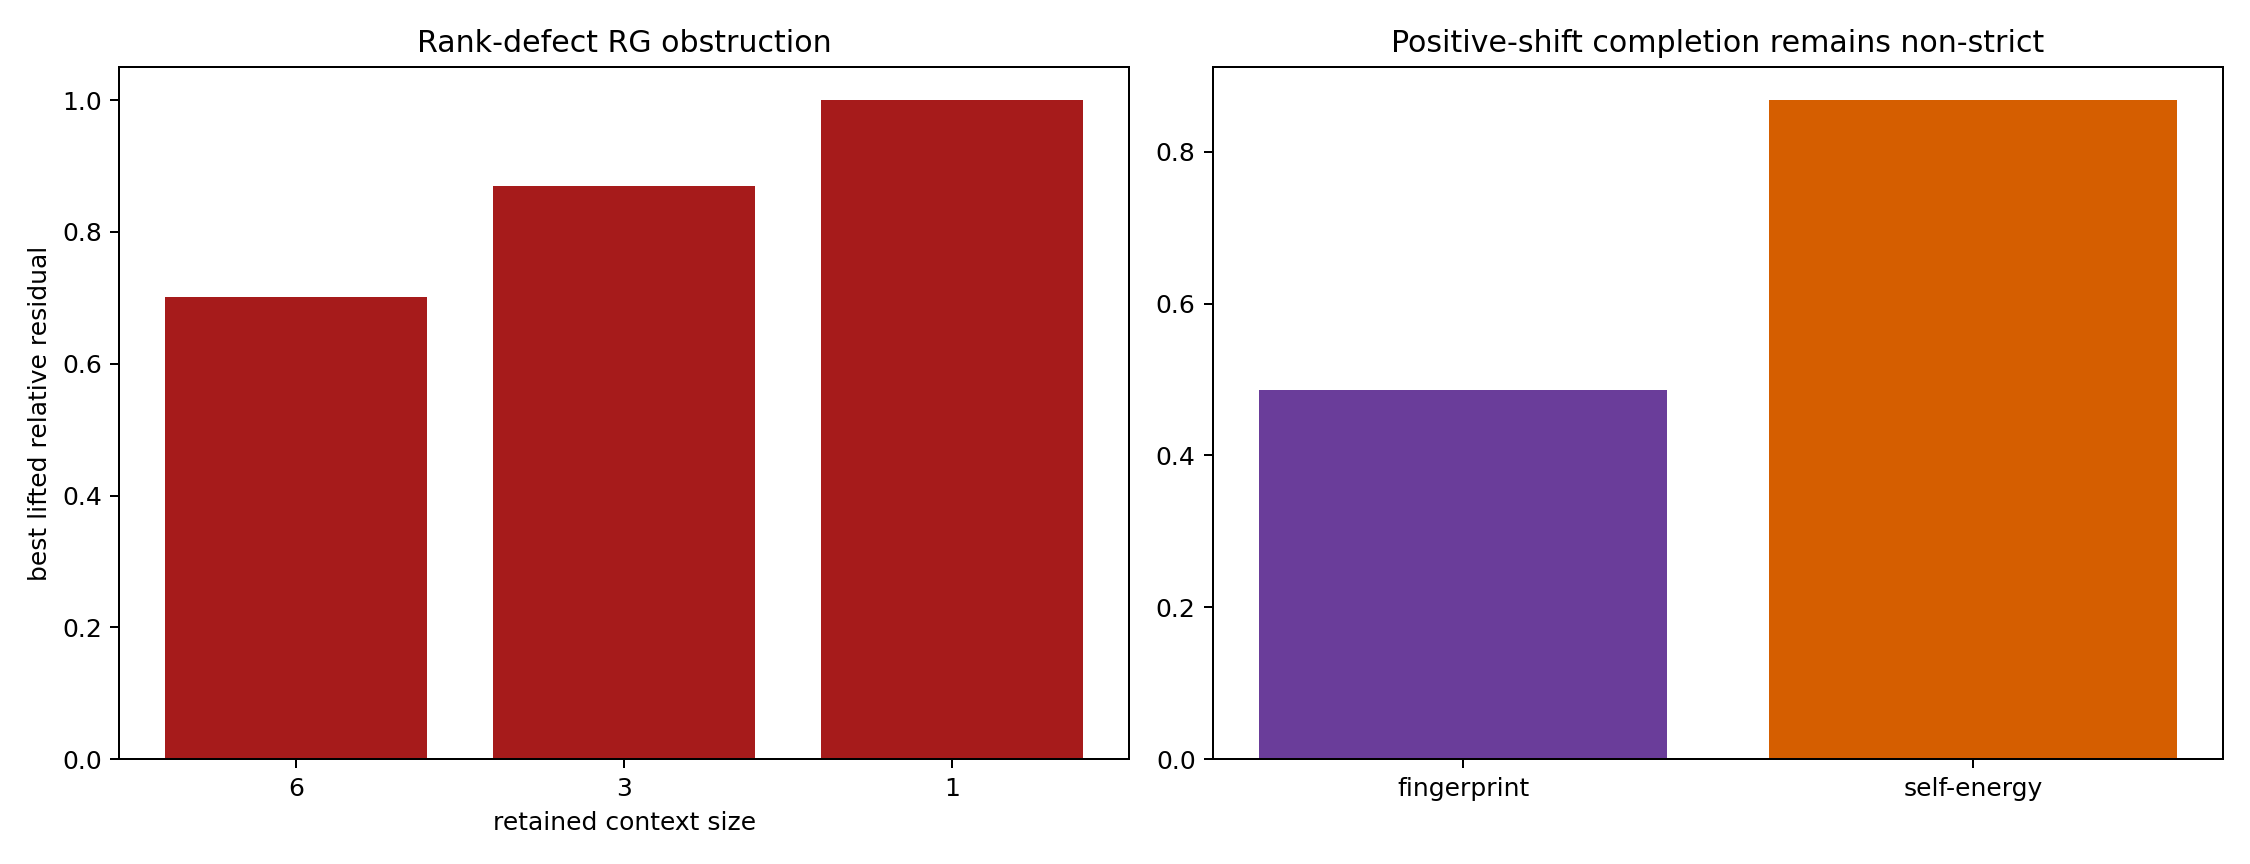
\includegraphics[width=0.97\textwidth]{FIN_Programs_267_280_Figures/p270_p272_rg_completion.png}
\caption{Rank-defect obstruction for linear size-restoring RG and the positive-shift legacy completion test.}
\end{figure}

\textbf{New missing object O29.} A nontrivial FIN renormalization comparison must take one of two forms:

\begin{enumerate}
\item 
a completion

\[
   \mathcal R(B_n)
   =
   EB_nE^\ast+C_\perp(B_n),
   \]

where \(C_\perp\) supplies dynamics on the missing complement; or

\item 
an observable quotient \(\pi\) for which

\[
   \pi(\mathcal R(B_n))
   \sim
   \pi(A_{\rm strict})
   \]

under a declared equivalence.

\end{enumerate}

Zero-padding and replication are excluded. A proposed complement may not be fitted after looking at the strict target without being marked as target-coded.

\chapter{P271 --- Quantum process-information ledger}

For a quantum instrument with Kraus operators \(\{K_y\}\), define

\[
p_y=\operatorname{tr}(K_y\rho K_y^\ast),\qquad
q_y=\operatorname{tr}(K_y\sigma K_y^\ast),
\]

and normalized conditional states

\[
\rho_y=\frac{K_y\rho K_y^\ast}{p_y},\qquad
\sigma_y=\frac{K_y\sigma K_y^\ast}{q_y}.
\]

The instrument channel with an explicit classical record is

\[
\Phi(\rho)
=
\bigoplus_y p_y\rho_y.
\]

Block-diagonal relative entropy gives

\[
D(\Phi(\rho)\Vert\Phi(\sigma))
=
D(p\Vert q)
+
\sum_y p_yD(\rho_y\Vert\sigma_y).
\]

Data processing gives the ledger

\[
\boxed{
D(\rho\Vert\sigma)
=
\mathcal L_{\rm inst}
+
D(p\Vert q)
+
\sum_y p_yD(\rho_y\Vert\sigma_y)
}
\]

with \(\mathcal L_{\rm inst}\ge0\).

Finite audit:

\begin{center}
\begingroup\small
\setlength{\tabcolsep}{2.5pt}
\renewcommand{\arraystretch}{1.16}
\begin{longtable}{@{}p{0.420\textwidth}p{0.420\textwidth}@{}}
\toprule
\textbf{Quantity} & \textbf{Result} \\
\midrule
\endhead
random state pairs & 400 \\
instrument completeness residual & 0 \\
minimum information loss & 0.0114899 nat \\
median information loss & 0.0830310 nat \\
maximum decomposition residual & \(2.22\times10^{-16}\) \\
\bottomrule
\end{longtable}
\endgroup
\end{center}

\textbf{Verdict.} This is the correct quantum extension of the earlier classical information ledger. It separates recorded distinguishability, conditional post-measurement distinguishability, and discarded information. The instrument is supplied. No FIN theorem presently derives the Hilbert space, Born probabilities, Kraus structure, laboratory detector, or environment.

\chapter{P272 --- One-atom legacy completion test}

The tested atom is the smallest uniform correction on the mean-zero sector:

\[
\Pi_0^\perp
=
I-\frac{\mathbf1\mathbf1^\top}{12},
\qquad
A_{\rm legacy}^{(+)}
=
A_{\rm legacy}+\gamma\Pi_0^\perp.
\]

Choose

\[
\gamma
=
\max\{0,-\lambda_{\min}
(A_{\rm legacy}|_{\mathbf1^\perp})\}
+10^{-9}.
\]

This uses legacy spectral data only. It gives:

\begin{center}
\begingroup\small
\setlength{\tabcolsep}{2.5pt}
\renewcommand{\arraystretch}{1.16}
\begin{longtable}{@{}p{0.420\textwidth}p{0.420\textwidth}@{}}
\toprule
\textbf{Quantity} & \textbf{Result} \\
\midrule
\endhead
legacy minimum mean-zero eigenvalue & \(-7.7101445443\) \\
derived \(\gamma\) & 7.7101445453 \\
completed minimum mean-zero eigenvalue & \(1.00\times10^{-9}\) \\
completed row-sum residual & \(1.99\times10^{-15}\) \\
strict projective fingerprint defect & 0.486509 \\
normalized self-energy defect at \(z=0.2\) & 0.867962 \\
\bottomrule
\end{longtable}
\endgroup
\end{center}

The correction moves legacy into the positive generator cone. It does not recover the strict spectral shape or strict context memory.

\textbf{Verdict.} Positivity is not the missing legacy-to-strict theorem. A uniform mass/\allowbreak{}shift correction is insufficient. No phase-frequency source, nonlinear compression exponent, target-independent damping source, selector, or physical role is obtained.

\chapter{P273 --- External-evidence admission gate}

The repository was searched for a production P241 transfer package satisfying the blind-custody contract.

\begin{center}
\begingroup\small
\setlength{\tabcolsep}{2.5pt}
\renewcommand{\arraystretch}{1.16}
\begin{longtable}{@{}p{0.420\textwidth}p{0.420\textwidth}@{}}
\toprule
\textbf{Requirement} & \textbf{Result} \\
\midrule
\endhead
production bundle\_manifest.json files & 0 \\
rows in heat-process template & 0 \\
rows in double-slit template & 0 \\
validator checks required & 11 \\
detached signature required & yes \\
P242 confirmatory execution authorized & no \\
\bottomrule
\end{longtable}
\endgroup
\end{center}

The absence of data is a scientifically meaningful outcome. The pipeline must not be run on synthetic replacements and described as experimental validation.

\textbf{Verdict.} A validator can certify syntax, hashes, signatures, frozen predictions, and role declarations. It cannot create independent preparation, provider/\allowbreak{}registrar/\allowbreak{}analyst separation, physical events, a trusted timestamp, or a laboratory signature.

\chapter{P274 --- Two-flux tomography and the noise-bias optimum}

Let \(\Sigma(\theta)\) be a flux-twisted self-energy and let

\[
\Xi
=
\left.\frac{\partial\Sigma(\theta)}
{\partial\theta}\right|_{\theta=0}.
\]

The centered estimator is

\[
\widehat\Xi_h
=
\frac{\widehat\Sigma(+h)-\widehat\Sigma(-h)}{2h}.
\]

Its deterministic bias is \(O(h^2)\), while independent measurement noise is amplified as \(O((h\sqrt N)^{-1})\). Consequently the total error must have an interior optimum.

The frozen synthetic audit used 50,000 shots per flux setting and fifteen values \(h\in[0.003,0.3]\).

\begin{center}
\begingroup\small
\setlength{\tabcolsep}{2.5pt}
\renewcommand{\arraystretch}{1.16}
\begin{longtable}{@{}p{0.420\textwidth}p{0.420\textwidth}@{}}
\toprule
\textbf{Quantity} & \textbf{Result} \\
\midrule
\endhead
tomography noise scale & 0.00156525 \\
optimal tested \(h\) & 0.11182781 \\
median relative error at optimum & 0.0115248 \\
95\% relative error at optimum & 0.0138276 \\
\bottomrule
\end{longtable}
\endgroup
\end{center}

At \(h=0.003\), noise amplification gives median relative error \(0.3706\). At the largest \(h\), truncation bias increases. The minimum between these regimes is therefore not an artifact of taking \(h\) as small as possible.

\textbf{Verdict.} The result supplies a rational experimental-design principle for chiral-memory tomography. The optimum is not universal: it depends on counts, contrast, detector response, drift, and the estimator. P288 must replace the matrix-Gaussian proxy by a platform-specific event likelihood.

\chapter{P275 --- Certified spectral-fingerprint exclusion}

Let

\[
f(A)
=
\frac{(\lambda_1,\ldots,\lambda_{11})}
{\lambda_{\max}}
\]

be the ordered nonzero spectral fingerprint of a connected positive generator. Suppose a null \(B\) is separated from the target by

\[
d=\|f(B)-f(A_{\rm strict})\|_2.
\]

For a Hermitian perturbation \(E\), Weyl's theorem and normalization give the bound

\[
\|f(B+E)-f(B)\|_2
\le
\frac{2\sqrt{11}\,\|E\|_2}
{\lambda_{\max}(B)-\|E\|_2},
\qquad
\|E\|_2<\lambda_{\max}(B).
\]

Thus a null remains outside a tolerance ball of radius \(\tau\) whenever

\[
\frac{2\sqrt{11}\,\epsilon}
{\lambda_{\max}(B)-\epsilon}
<
d-\tau.
\]

Frozen audit:

\begin{center}
\begingroup\small
\setlength{\tabcolsep}{2.5pt}
\renewcommand{\arraystretch}{1.16}
\begin{longtable}{@{}p{0.420\textwidth}p{0.420\textwidth}@{}}
\toprule
\textbf{Quantity} & \textbf{Result} \\
\midrule
\endhead
positive-circulant nulls & 400 \\
tolerance & 0.02 \\
false positives & 0 \\
minimum fingerprint distance & 0.121302 \\
median fingerprint distance & 0.535086 \\
minimum positive certified radius & 0.102825 \\
median certified radius & 0.404749 \\
\bottomrule
\end{longtable}
\endgroup
\end{center}

\begin{figure}[htbp]
\centering
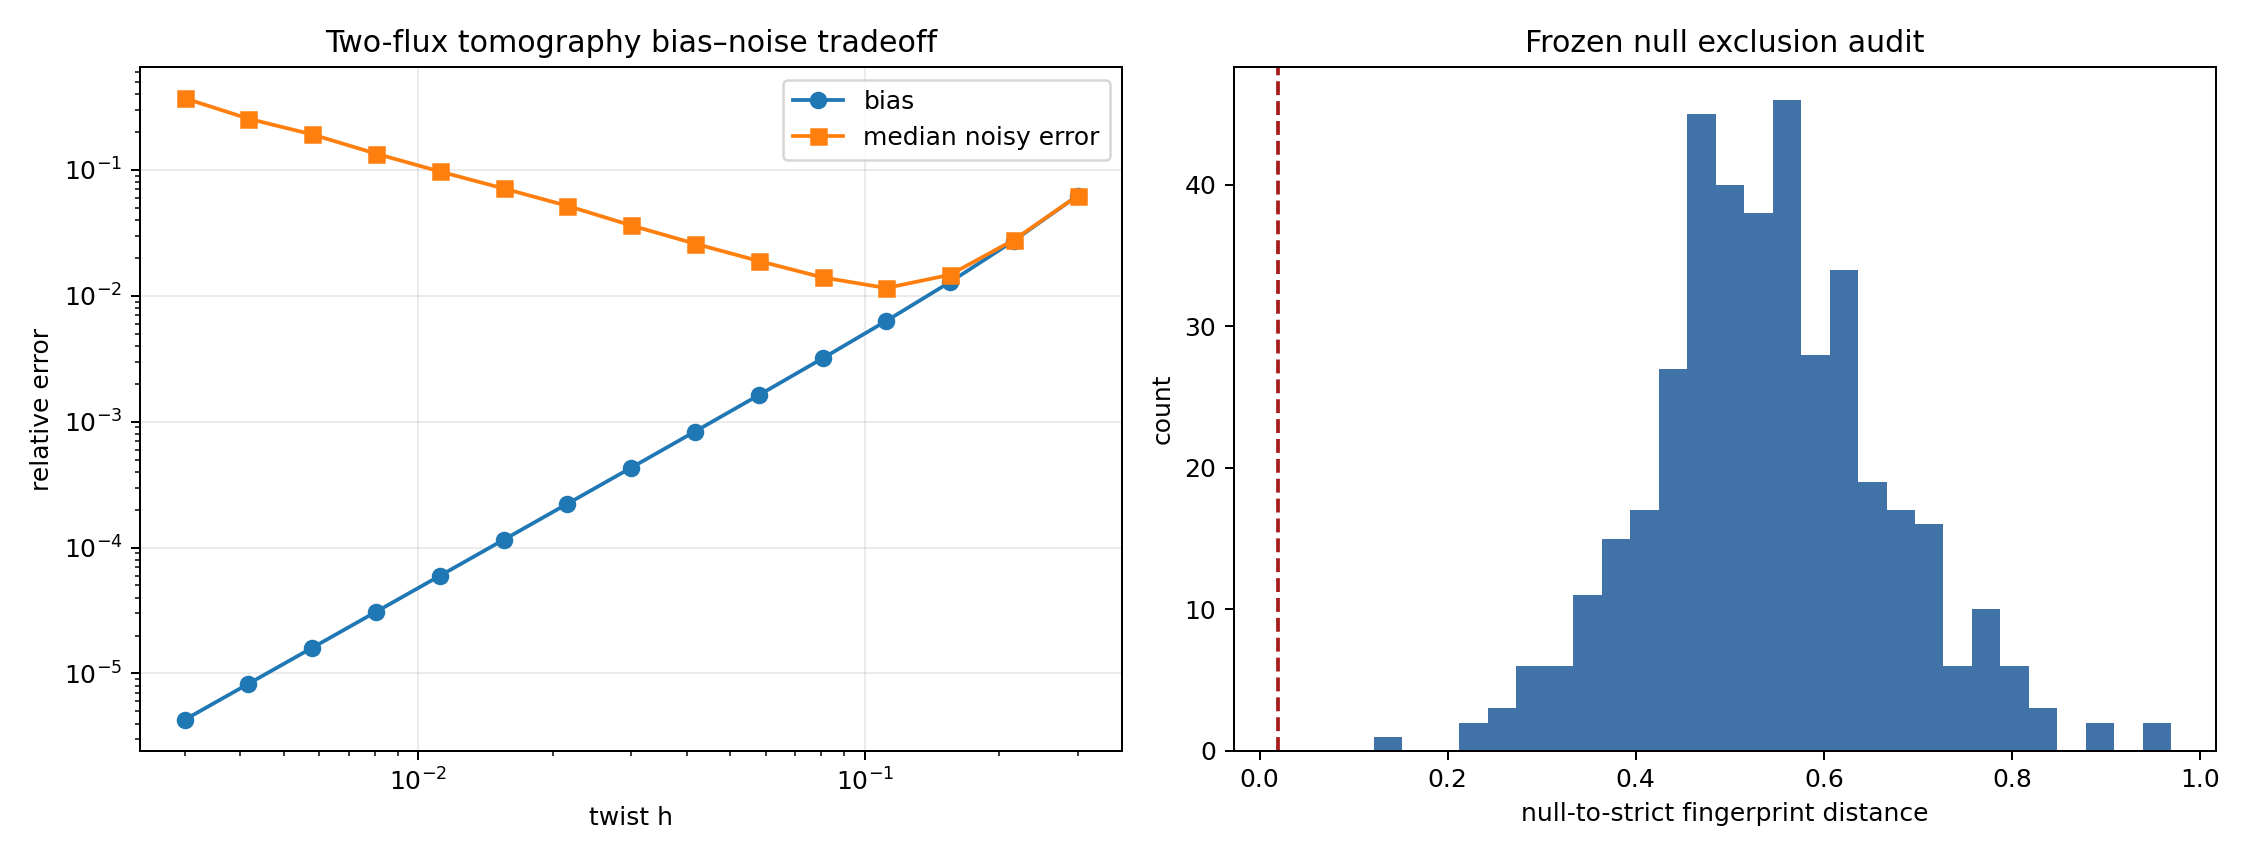
\includegraphics[width=0.97\textwidth]{FIN_Programs_267_280_Figures/p274_p275_tomography_false_positive.png}
\caption{Finite-flux bias--noise optimization and deterministic robustness certificates for the frozen null fingerprints.}
\end{figure}

\textbf{Verdict.} Every frozen null has a nonzero deterministic robustness certificate. The theorem is stronger than a sample-only observation but narrower than an ensemble-level false-positive probability. It says nothing about null families not represented in the frozen set.

\chapter{P276 --- Calibrated two-time semigroup consistency}

Let \(P_1,P_2\) be symmetric positive-definite transition matrices observed at calibrated times \(0<t_1<t_2\).

\textbf{Theorem P276.} There exists a homogeneous symmetric positive-semidefinite generator \(A\) such that

\[
P_1=e^{-t_1A},\qquad P_2=e^{-t_2A}
\]

if and only if:

\begin{enumerate}
\item 
\(P_1P_2=P_2P_1\);

\item 
\(\log(P_1)/t_1=\log(P_2)/t_2\);

\item 
\(-\log(P_1)/t_1\succeq0\).

\end{enumerate}

When it exists, \(A=-\log(P_1)/t_1\) is unique.

The frozen times were \(t_1=0.20\) and \(t_2=0.55\).

\begin{center}
\begingroup\small
\setlength{\tabcolsep}{2.5pt}
\renewcommand{\arraystretch}{1.16}
\begin{longtable}{@{}p{0.314\textwidth}p{0.285\textwidth}p{0.261\textwidth}@{}}
\toprule
\textbf{Mechanism} & \textbf{Relative log-generator defect} & \textbf{Commutator residual} \\
\midrule
\endhead
static FIN generator & \(1.84\times10^{-15}\) & \(1.36\times10^{-16}\) \\
uniform scale with calibrated clock & \(1.76\times10^{-15}\) & numerical zero \\
generator-shape drift & 0.0540739 & 0.0085286 \\
mixture-memory map & 0.0184292 & 0.0039854 \\
\bottomrule
\end{longtable}
\endgroup
\end{center}

There is also an exact uncalibrated degeneracy:

\[
e^{-t(cA)}=e^{-(ct)A},
\]

with residual \(2.29\times10^{-16}\) in the audit.

\textbf{Verdict.} Calibrated multitime data can falsify homogeneous FIN evolution. Two time slices do not identify whether a failure was caused by adaptive dynamics, an uncontrolled bath, time-dependent hardware, or apparatus memory. At least one more time slice and causal interventions are needed.

\chapter{P277 --- Intervention-identifiable adaptive law}

Four candidate laws were frozen:

\[
\dot w=0,
\]

\[
\dot w=-\kappa(w-w_0),
\]

\[
\dot w=-\kappa(w-w_0)+g\,u(t)d,
\]

\[
\dot w=w\odot[-\kappa\mathbf1+g\,u(t)d].
\]

The synthetic truth was the driven additive law with

\[
(\kappa,g)=(0.24,0.075).
\]

Without intervention, the design matrix has rank one. With a signed control sequence \(u(t)\), its rank rises to two. The fitted winning parameters were

\[
(\widehat\kappa,\widehat g)
=
(0.24037046,0.0750176).
\]

\begin{center}
\begingroup\small
\setlength{\tabcolsep}{2.5pt}
\renewcommand{\arraystretch}{1.16}
\begin{longtable}{@{}p{0.420\textwidth}p{0.420\textwidth}@{}}
\toprule
\textbf{Candidate} & \textbf{Hold-out MSE} \\
\midrule
\endhead
driven additive & \(2.83\times10^{-10}\) \\
static & \(3.88\times10^{-4}\) \\
relaxation & \(4.17\times10^{-4}\) \\
multiplicative & \(1.16\times10^{-3}\) \\
\bottomrule
\end{longtable}
\endgroup
\end{center}

\textbf{Verdict.} Interventions can turn an observationally underidentified adaptive model into an identifiable one. This is a systems-identification result. The candidate panel, forcing direction, and input are supplied; no strict FIN theorem presently selects this adaptive law.

\chapter{P278 --- Nonlinear matched reservoir benchmark}

The nonlinear update was

\[
x_{t+1}
=
\tanh(Rx_t+b\,u_t),
\qquad
R_{\rm FIN}=0.92\,e^{-0.25A}.
\]

FIN was compared with thirty isospectral random-orientation controls and thirty symmetric spectral-radius-matched controls on four frozen tasks.

\begin{center}
\begingroup\small
\setlength{\tabcolsep}{2.5pt}
\renewcommand{\arraystretch}{1.16}
\begin{longtable}{@{}p{0.322\textwidth}p{0.212\textwidth}p{0.326\textwidth}@{}}
\toprule
\textbf{Task} & \textbf{FIN score} & \textbf{FIN percentile among controls} \\
\midrule
\endhead
delay-5 \(R^2\) & 0.247307 & 0.4167 \\
nonlinear prediction \(R^2\) & 0.710659 & 0.3000 \\
NARMA10 \(R^2\) & 0.686674 & 1.0000 \\
parity-3 accuracy & 0.754706 & 0.0667 \\
\bottomrule
\end{longtable}
\endgroup
\end{center}

FIN exceeds every control on one of four tasks: NARMA10. The best control achieves \(R^2=0.683686\), only about \(0.0030\) below FIN.

\begin{figure}[htbp]
\centering
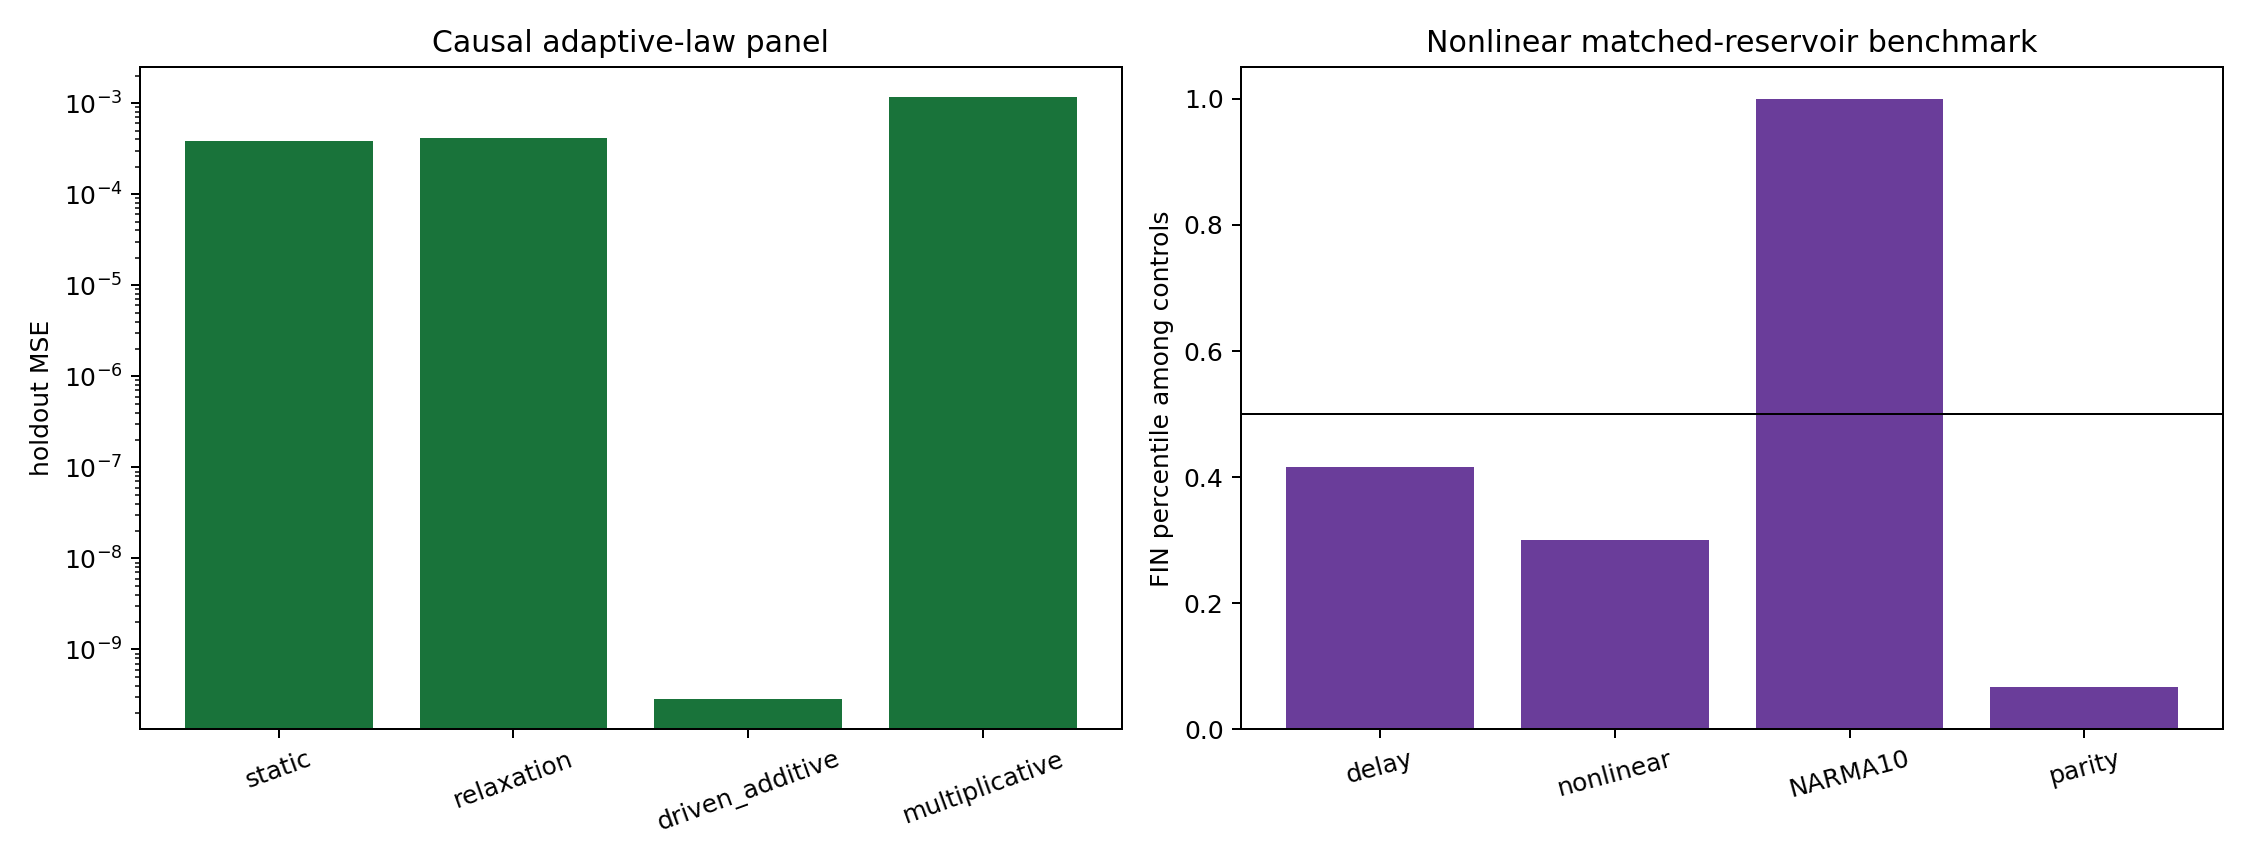
\includegraphics[width=0.97\textwidth]{FIN_Programs_267_280_Figures/p277_p278_adaptation_reservoir.png}
\caption{Intervention-based adaptive-law discrimination and the nonlinear matched-reservoir task benchmark.}
\end{figure}

\textbf{Verdict.} The new nonlinear audit is more favorable than the earlier linear-memory benchmark, but only in a task-specific sense. Four outcomes were inspected, the margin is small, and the study uses one frozen input realization. No general claim about intelligence, biological memory, optimal computation, or physical implementation is warranted.

\chapter{P279 --- Conditional information-to-energy conversion}

Let

\[
\gamma=\frac{e^{-\beta H}}{Z},\qquad
\beta=(k_BT)^{-1},
\]

and

\[
F(\rho)=\operatorname{tr}(\rho H)-k_BT\,S(\rho).
\]

Then

\[
\begin{aligned}
D(\rho\Vert\gamma)
&=
\operatorname{tr}(\rho\log\rho)
-\operatorname{tr}(\rho\log\gamma)\\
&=
-S(\rho)+\beta\operatorname{tr}(\rho H)+\log Z\\
&=
\beta\bigl(F(\rho)-F(\gamma)\bigr).
\end{aligned}
\]

This is the precise bridge from relative information to nonequilibrium free energy.

The frozen conditional example supplied:

\[
\Delta H=1.3,\qquad T=2,\qquad k_B=1,
\]

and a \(37\%\) thermalizing mixture.

\begin{center}
\begingroup\small
\setlength{\tabcolsep}{2.5pt}
\renewcommand{\arraystretch}{1.16}
\begin{longtable}{@{}p{0.420\textwidth}p{0.420\textwidth}@{}}
\toprule
\textbf{Quantity} & \textbf{Result} \\
\midrule
\endhead
\(D(\rho\Vert\gamma)\) before & 0.0805837 nat \\
after & 0.0310255 nat \\
information decrease & 0.0495583 nat \\
free-energy decrease & 0.0991165 \\
identity residual & \(1.7\times10^{-16}\) \\
conversion residual & \(1.94\times10^{-16}\) \\
one-bit Landauer scale \(k_BT\ln2\) & 1.386294 \\
\bottomrule
\end{longtable}
\endgroup
\end{center}

The conversion is

\[
\Delta F=k_BT\,\Delta D
\]

for the stated Gibbs reference and supplied dimensional constants.

\textbf{Verdict.} Information does not become energy by notation alone. The Hamiltonian identifies what counts as energy; the temperature identifies the conversion scale; \(k_B\) converts dimensionless entropy to physical entropy. FIN currently supplies none of these dimensionful resources internally. The identity is a valid conditional functor from an information ledger to a thermodynamic ledger.

\chapter{P280 --- Product torsor for scale and orientation}

Let

\[
\mathcal T_{\rm scale}\cong\mathbb R_{>0}
\]

be the set of positive scale choices, and let

\[
\mathcal T_{\rm orient}\cong\mathbb Z_2
\]

be the two orientation choices. Their product acts as

\[
(\kappa,\varepsilon):
(A,J)
\longmapsto
(\kappa A,\varepsilon J).
\]

An operational section is

\[
s=(\kappa,\varepsilon)
\in
\mathcal T_{\rm scale}\times\mathcal T_{\rm orient}.
\]

The spectral fingerprint is invariant under \(\kappa\), while the directed current changes sign under \(\varepsilon\). The audit used scales \(0.5\) and \(1.7\), and both signs.

\begin{center}
\begingroup\small
\setlength{\tabcolsep}{2.5pt}
\renewcommand{\arraystretch}{1.16}
\begin{longtable}{@{}p{0.420\textwidth}p{0.420\textwidth}@{}}
\toprule
\textbf{Quantity} & \textbf{Residual} \\
\midrule
\endhead
scale-fingerprint invariance & \(8.27\times10^{-16}\) \\
orientation sign pairing & 0 \\
time reparameterization & at most \(3.57\times10^{-16}\) \\
\bottomrule
\end{longtable}
\endgroup
\end{center}

\begin{figure}[htbp]
\centering
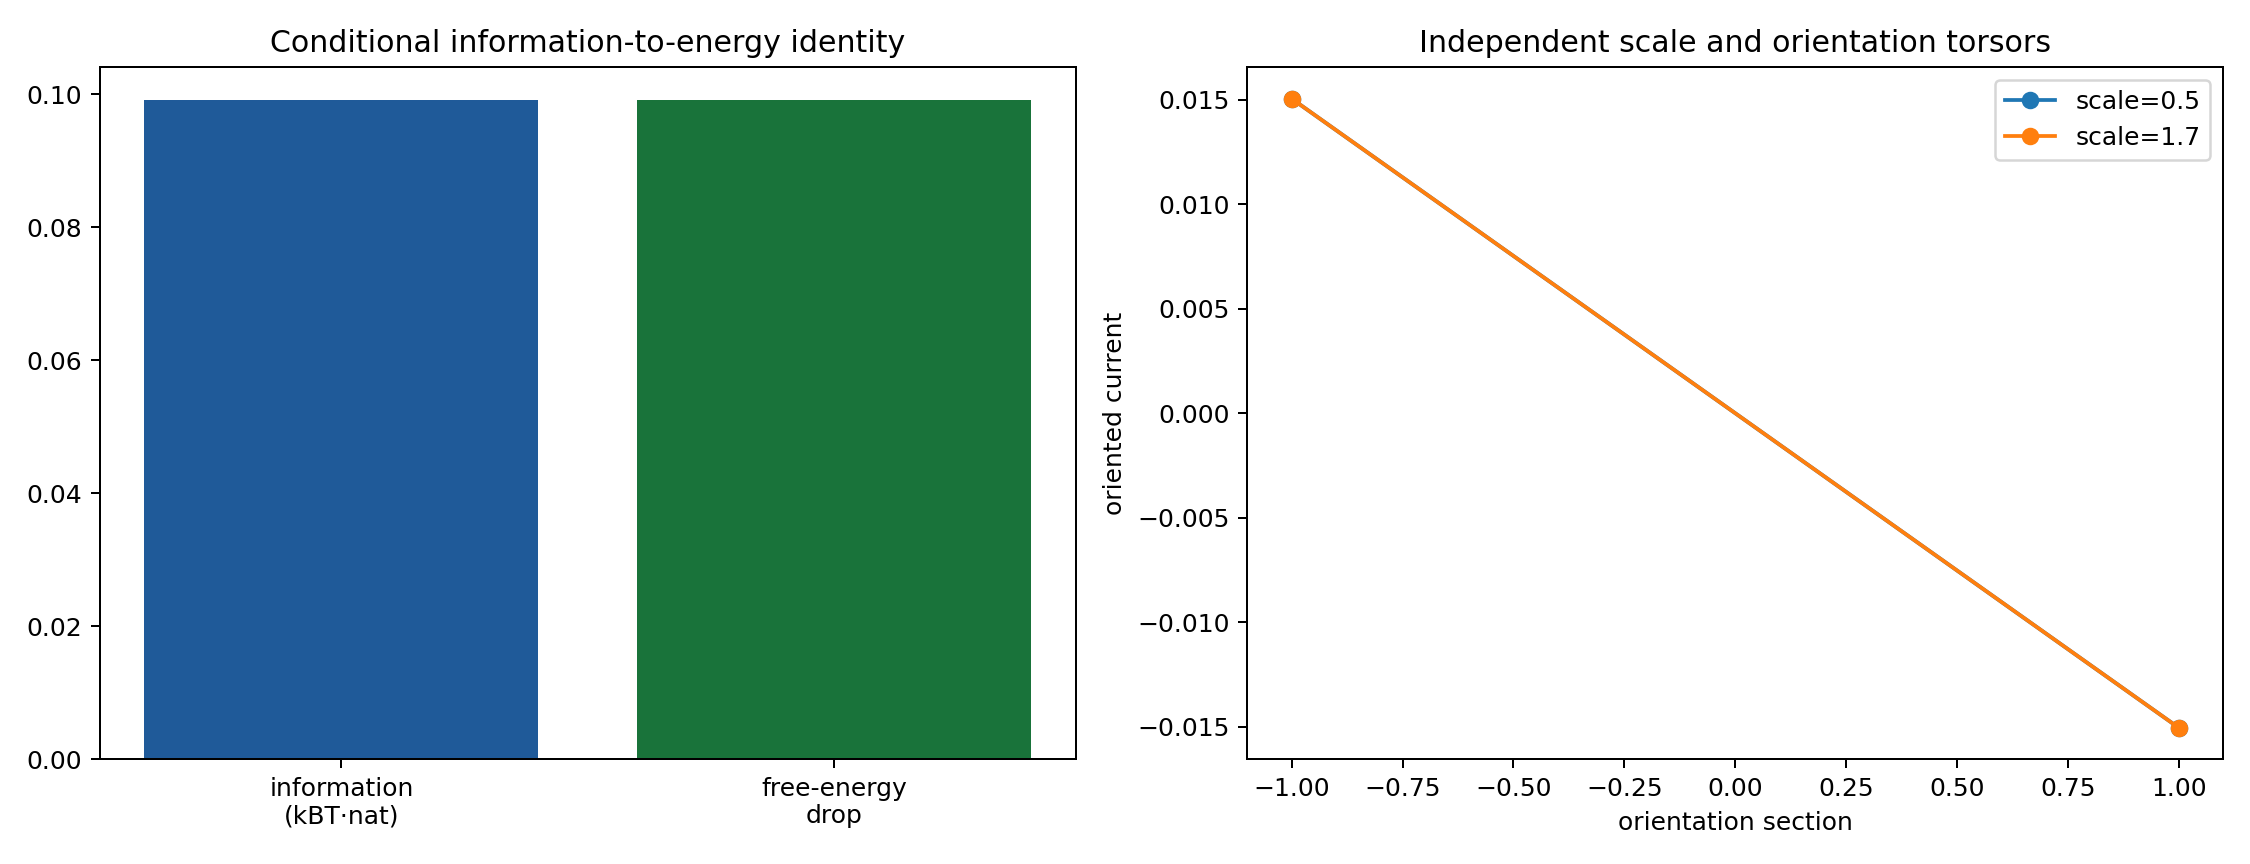
\includegraphics[width=0.97\textwidth]{FIN_Programs_267_280_Figures/p279_p280_conversion_torsors.png}
\caption{Conditional conversion from relative information to free energy and the independent scale--orientation product torsor.}
\end{figure}

\textbf{Independence theorem.} Positive rescaling cannot choose a \(\mathbb Z_2\) orientation, and orientation reversal cannot set a positive dimensional scale. Therefore the two obstructions are independent unless a new theorem couples them through an additional nontrivial object.

\textbf{Verdict.} The product torsor is the cleanest present description of FIN's two most persistent missing resources. A chosen section is an operational completion, not an emergent selector or unit theorem.

\chapter{Newly constructed theoretical objects O26--O39}

\begin{center}
\begingroup\small
\setlength{\tabcolsep}{2.5pt}
\renewcommand{\arraystretch}{1.16}
\begin{longtable}{@{}p{0.289\textwidth}p{0.195\textwidth}p{0.258\textwidth}p{0.117\textwidth}@{}}
\toprule
\textbf{Object} & \textbf{Definition} & \textbf{What it explains} & \textbf{Status} \\
\midrule
\endhead
O26 Visible Stieltjes Measure Certificate & poles and nonzero residue matrices of \(\Sigma_E\), with uncertainty model & exact visible-memory identity and inverse instability & \statusProven{} /\allowbreak{} \statusStrong{} \\
O27 Executable Schur Category Core & contexts, unique inclusions, Schur morphisms, identities, composition, positivity & functorial context reduction & \statusProven{} \\
O28 Minimal Six-Outcome Current POVM & simplex perturbations of \(I/6\) in the five-current subspace & smallest one-shot informational current readout & \statusProven{} \\
O29 Rank-Defect RG Obstruction & \(\operatorname{rank}(EBE^\ast)\le n-1<11\) & why simple lifting cannot restore \(Z_{12}\) & \statusProven{} \\
O30 Quantum Process Information Ledger & record divergence + conditional quantum divergence + loss & information accounting through instruments & \statusProven{}, conditional \\
O31 Positive-Shift Completion Atom & \(A_{\rm legacy}+\gamma\Pi_0^\perp\) & separates cone repair from kernel completion & \statusProven{} \\
O32 External-Evidence Admission Certificate & hashes, signature, roles, frozen hold-out, event-row and manifest checks & boundary between executable code and empirical independence & Executed \\
O33 Two-Flux Noise-Bias Tomography Design & centered derivative estimator with optimized \(h\) & finite-count design for chiral response & \statusStrong{} \\
O34 Certified Fingerprint Exclusion Radius & perturbation radius derived from eigenvalue stability & robust exclusion for each frozen null & \statusProven{} \\
O35 Two-Time Semigroup Consistency Object & commutator plus equality of calibrated log generators & falsification of homogeneous dynamics & \statusProven{} \\
O36 Intervention-Identifiable Adaptive Panel & finite law family + full-rank input design + hold-out & separates passive fit from causal identifiability & \statusProven{} /\allowbreak{} \statusStrong{} \\
O37 Nonlinear Matched Reservoir Null Benchmark & task battery with isospectral and radius-matched controls & tests whether FIN geometry adds computational value & \statusStrong{} \\
O38 Thermodynamic Conversion Functor & \((\rho,\gamma,H,T,k_B)\mapsto F\) via relative entropy & exact conditional information-to-energy map & \statusProven{}, conditional \\
O39 Product-Torsor Operational Section & \(s=(\kappa,\varepsilon)\in\mathbb R_{>0}\times\mathbb Z_2\) & organizes independent scale and orientation resources & \statusProven{}, conditional \\
\bottomrule
\end{longtable}
\endgroup
\end{center}

These objects are not fourteen new forces or physical entities. They are minimal mathematical interfaces that either close a precisely stated subproblem or expose the exact premise still missing.

\chapter{Falsification matrix}

\begin{center}
\begingroup\small
\setlength{\tabcolsep}{2.5pt}
\renewcommand{\arraystretch}{1.16}
\begin{longtable}{@{}p{0.222\textwidth}p{0.213\textwidth}p{0.213\textwidth}p{0.213\textwidth}@{}}
\toprule
\textbf{Proposed bridge} & \textbf{Destructive test} & \textbf{Outcome} & \textbf{Surviving statement} \\
\midrule
\endhead
exact self-energy determines hidden physics & add invisible modes or perturb pole data & microscopic realization nonunique; inverse unstable & exact visible measure is unique \\
context reductions imply a complete categorical physics & demand proof-assistant kernel and gluing law & not supplied & finite Schur category core survives \\
vertex data suffice for FIN currents & conjugate states with equal populations and opposite currents; construct POVM & vertex-only claim fails; six-outcome current POVM exists abstractly & current readout requires phase-sensitive instrument \\
simple lifting creates an RG fixed point & rank comparison & impossible for \(n<12\) & complement dynamics or quotient equivalence required \\
process information is already thermodynamics & remove \(H,T,k_B\) & energy scale disappears & quantum information ledger survives \\
uniform legacy correction yields strict & compare fingerprint and self-energy & defects 0.4865 and 0.8680 & positivity repair only \\
pipeline code validates physics & search for external signed P241 package & no production package & no-admission certificate \\
arbitrarily small flux is optimal & finite-count noise amplification & false & interior bias-noise optimum \\
zero sampled false positives proves uniqueness & perturb each null and ask for ensemble theorem & only local finite certificates obtained & 400 robust exclusions \\
two time slices reveal the cause of non-Markovianity & compare drift and mixtures & both can fail test & homogeneous semigroup is falsifiable, cause is not identified \\
observational adaptation fit identifies the law & remove interventions & design rank drops from 2 to 1 & controlled finite-family selection works \\
FIN is a generally superior reservoir & compare four tasks and matched controls & advantage on only 1/\allowbreak{}4 tasks & task-specific NARMA10 result \\
information fixes energy scale & rescale \(H\), \(T\), or \(k_B\) & dimensional answer changes & Gibbs free-energy identity is conditional \\
scale selection fixes orientation & act independently by \(\mathbb R_{>0}\) and \(\mathbb Z_2\) & no cross-selection & product-torsor description survives \\
\bottomrule
\end{longtable}
\endgroup
\end{center}

\chapter{Current state of the theory}

\section{What is established}

The following core survives all present falsification attempts:

\begin{enumerate}
\item 
A finite self-adjoint graph generator \(A\) exists and produces unitary and diffusive semigroups.

\item 
Its Green/\allowbreak{}resolvent family and context self-energies are consequences of the spectral theorem and Schur reduction.

\item 
Every proper context carries a finite positive operator-valued Stieltjes memory measure.

\item 
Context reduction composes exactly and preserves positivity.

\item 
The visible input-output memory realization is identifiable only up to invisible modes and realization equivalence.

\item 
Chiral or current observables require phase-sensitive operational access.

\item 
Information loss can be rigorously tracked through classical or quantum instruments.

\item 
Physical energy can be attached consistently once a Hamiltonian, temperature, and conversion constant are supplied.

\end{enumerate}

This is a coherent mathematical research program in finite spectral operator theory, reduced dynamics, information processing, and operational identifiability.

\section{What remains conditional}

The following structures can be built consistently but are not selected by the strict kernel:

\begin{itemize}
\item 
a current POVM;

\item 
a quantum instrument;

\item 
a thermal reference and bath;

\item 
a dimensional calibration;

\item 
an adaptive law and intervention channel;

\item 
an RG complement or observable quotient;

\item 
an orientation section;

\item 
a laboratory platform.

\end{itemize}

Their consistency is valuable: it shows that no immediate algebraic contradiction prevents physicalization. Their nonuniqueness is equally important: the strict spectrum does not force one of them.

\section{What is presently blocked}

The following remain blocked on current artifacts:

\begin{itemize}
\item 
non-premise selector closure and discharge of QW-2191;

\item 
canonical length/\allowbreak{}UV unit;

\item 
target-independent strict damping/\allowbreak{}compression source;

\item 
role-safe legacy amplitude transfer;

\item 
full legacy-to-strict completion map;

\item 
strict tensor-resolved Lagrangian/\allowbreak{}EOM reverse closure;

\item 
role-bearing total action;

\item 
experimentally trusted P241 data;

\item 
unique physical interpretation.

\end{itemize}

\section{Quantitative classification}

Scores use a 0--5 scale and assess the current repository, not its ambition.

\begin{center}
\begingroup\small
\setlength{\tabcolsep}{2.5pt}
\renewcommand{\arraystretch}{1.16}
\begin{longtable}{@{}p{0.392\textwidth}p{0.086\textwidth}p{0.382\textwidth}@{}}
\toprule
\textbf{Interpretation} & \textbf{Score} & \textbf{Reason} \\
\midrule
\endhead
finite spectral operator theory & 4.8 & exact generator, resolvent, functional calculus, spectral fingerprints \\
context-dependent reduced dynamics & 4.7 & exact Schur memory and positive operator measures \\
information-process theory & 4.3 & classical and quantum distinguishability ledgers, operational records \\
graph signal processing /\allowbreak{} quantum-walk substrate & 4.1 & \(Z_{12}\) graph, filters, currents, unitary and heat evolution \\
adaptive computation /\allowbreak{} reservoir model & 3.1 & valid supplied laws and benchmarks, but no strict source law or general advantage \\
noncommutative/\allowbreak{}spectral geometry & 2.9 & finite spectral ingredients exist; full geometric/\allowbreak{}physical axioms are not forced \\
statistical mechanics & 2.5 & exact conditional Gibbs bridge, no internally generated \(H,T,k_B\) \\
field theory & 2.0 & propagator/\allowbreak{}action reconstructions are conditional and finite \\
self-referential dynamical system & 1.8 & adaptive feedback can be supplied; strict bootstrap uniqueness remains absent \\
experimentally predictive physical theory & 1.3 & test contracts exist, independent data and dimensional map do not \\
Theory of Everything & 0.0 & not established and outside the valid mathematical conclusions \\
\bottomrule
\end{longtable}
\endgroup
\end{center}

\section{Deepest surviving interpretation}

The deepest present interpretation is:

\begin{quote}\itshape
\textbf{FIN is a finite spectral information-processing system whose apparent Green functions, kernels, memory, wave dynamics, diffusion, variational forms, and operational information ledgers are different representations or reductions of a positive self-adjoint generator together with chosen contexts. Physical meaning enters only after additional operational, dimensional, and symmetry-breaking resources are supplied.}

\end{quote}

The underlying mathematical unifier is therefore not a new physical law at present. It is the pair

\[
\boxed{(A,\mathcal C)}
\]

where \(A\) is the positive spectral generator and \(\mathcal C\) is the category of accessible contexts and Schur reductions. The smallest operational extension is

\[
\boxed{(A,\mathcal C,\mathfrak O)}.
\]

A physical theory requires at least

\[
\boxed{(A,\mathcal C,\mathfrak O,\mathfrak C,\mathfrak S)}
\]

plus empirical evidence that one concrete realization obeys the specified predictions.

\chapter{The smallest missing theorem}

A single theorem connecting spectral operator, information, dynamics, dimensional physics, and observables would need to establish all of the following from strict FIN data alone:

\begin{enumerate}
\item 
a state functor assigning physical states to the spectral object;

\item 
a non-premise clock and dimensional calibration;

\item 
a unique physical instrument or equivalence class of instruments;

\item 
a signed orientation/\allowbreak{}selector;

\item 
a Hamiltonian or action with fixed physical dimensions;

\item 
a map from mathematical probabilities to event-level observables;

\item 
stability and universality under coarse graining;

\item 
at least one parameter-free empirical prediction.

\end{enumerate}

P267--P280 show that no theorem based only on spectral uniqueness, linear lifting, positivity repair, information monotonicity, or torsor bookkeeping can do this.

There is also a general dimensional obstruction:

\textbf{Scale-orbit obstruction.} Let every strict input be dimensionless and let the strict equations be equivariant under

\[
A\mapsto cA,\qquad t\mapsto t/c,\qquad c>0.
\]

Then no equivariant construction from those inputs alone can select a unique nonzero dimensional time or energy scale. Any such selection must either:

\begin{itemize}
\item 
introduce a dimensionful datum;

\item 
choose a gauge/\allowbreak{}section of the scale orbit;

\item 
invoke a boundary condition or empirical calibration that breaks the symmetry.

\end{itemize}

Likewise, if the strict data are invariant under orientation reversal, no equivariant scalar functional can select one of the two orientations. P280 shows that the two missing sections are independent.

Therefore the plausible "missing theorem" is not a theorem of the current strict object alone. It would have to be a theorem about an enlarged object carrying additional resource data. A scientifically honest target is:

\begin{quote}\itshape
\textbf{Operational Physicalization Theorem (candidate).} Given a strict spectral system, a calibrated conversion resource, a signed symmetry-breaking resource, and an informationally complete instrument satisfying declared compatibility and stability axioms, construct a unique empirical model up to operational equivalence, and prove robust parameter-free predictions.

\end{quote}

This candidate is not yet proven. Its value is that every indispensable input is visible rather than hidden in interpretation.

\chapter{Relation to existing mathematics and physics}

\section{Stieltjes and realization theory}

The positive-resolvent representation belongs to classical operator-valued Stieltjes/\allowbreak{}Nevanlinna theory. FIN's distinctive feature is not the existence of such a representation, but its use as a unified description of finite context memory and its connection to the frozen strict fingerprint. The visible/\allowbreak{}invisible realization quotient is standard in spirit: transfer functions determine only minimal controllable-observable realizations.

\section{Kron reduction and Schur complements}

Eliminating hidden vertices by a Schur complement is mathematically the same operation that appears in Kron reduction of electrical networks. FIN adds a frequency-dependent self-energy and interprets it as informational memory. That interpretation is compatible with the mathematics but does not make the Schur complement novel by itself.

\section{Quantum tomography and process tensors}

The six-outcome simplex POVM is an instance of informational design in a restricted observable subspace. It is not a full \(12\)-dimensional informationally complete POVM. The process ledger is a one-step quantum instrument statement; process-tensor tomography is the appropriate comparison for multitime, non-Markovian laboratory data.

\section{Mori-Zwanzig and open systems}

The FIN self-energy is a finite resolvent realization of the same broad mechanism that projection-operator methods express as memory kernels and fluctuating forces. FIN currently supplies an exact finite matrix representation. It does not yet derive a physical bath, fluctuation-dissipation relation, or thermodynamic noise source.

\section{Reservoir computing}

The adaptive and nonlinear benchmarks place FIN near reservoir computing and system identification. The NARMA10 result is a valid frozen synthetic finding, not evidence for a universal computational advantage. Multiple seeds, independent controls, hardware constraints, and correction for task selection are still needed.

\section{Landauer and resource-theoretic thermodynamics}

Landauer-type bounds and Gibbs-relative-entropy identities explain how dimensionless information acquires an energetic meaning once the physical resource theory is specified. They do not derive \(k_B\), \(T\), a Hamiltonian, or a reset protocol from Shannon information.

\section{Principal literature anchors}

\begin{itemize}
\item 
S. Belyi and E. Tsekanovskii, \href{https://arxiv.org/abs/0708.0452}{realization theory for operator-valued Stieltjes functions and conservative systems}.

\item 
F. Dörfler and F. Bullo, \href{https://arxiv.org/abs/1102.2950}{\emph{Kron Reduction of Graphs with Applications to Electrical Networks}}.

\item 
S. T. Flammia, A. Silberfarb, and C. M. Caves, \href{https://arxiv.org/abs/quant-ph/0404137}{\emph{Minimal Informationally Complete Measurements for Pure States}}.

\item 
F. A. Pollock et al., \href{https://arxiv.org/abs/1512.00589}{the process-tensor framework for operational non-Markovian quantum processes}.

\item 
R. Reeb and M. M. Wolf, \href{https://arxiv.org/abs/1306.4352}{\emph{An Improved Landauer Principle with Finite-Size Corrections}}.

\item 
H. Jaeger, \href{https://publica.fraunhofer.de/entities/publication/9dfaead1-4dc0-4e3c-b89b-596f50f671c1}{foundational work on echo-state/\allowbreak{}reservoir computing}.

\end{itemize}

These comparisons constrain originality claims. The present novelty, if any, must lie in a rigorously specified integration of the strict FIN fingerprint, context memory, operational tests, and resource boundaries---not in renaming standard spectral, Schur, tomography, or thermodynamic identities.

\chapter{Recommended Programs P281--P294}

The next programs are ranked by expected proof value, falsifiability, and ability to unlock a genuinely new frontier without replaying closed lanes.

\section{Priority table}

\begin{center}
\begingroup\fontsize{7}{8.4}\selectfont
\setlength{\tabcolsep}{2.5pt}
\renewcommand{\arraystretch}{1.16}
\begin{longtable}{@{}p{0.055\textwidth}p{0.088\textwidth}p{0.286\textwidth}p{0.277\textwidth}p{0.154\textwidth}@{}}
\toprule
\textbf{Rank} & \textbf{Program} & \textbf{Research objective} & \textbf{Success criterion} & \textbf{Estimated probability} \\
\midrule
\endhead
1 & P281 & minimax-stable Stieltjes inversion & rigorous error bounds and regularized recovery region & 0.75 \\
2 & P290 & three-time causal separation of drift and memory & identifiable mechanism classes under frozen interventions & 0.70 \\
3 & P283 & hardware-realizable six-outcome current POVM & detector likelihood, calibration matrix, uncertainty budget & 0.65 \\
4 & P289 & ensemble-level fingerprint false-positive theorem & analytic or importance-sampled tail probability & 0.60 \\
5 & P282 & proof-assistant Schur category & machine-checked identities, composition, positivity & 0.85 \\
6 & P285 & multitime quantum process ledger & process-tensor chain rule and data-processing certificate & 0.65 \\
7 & P291 & optimal intervention design for adaptive laws & full-rank Fisher information with minimal controls & 0.70 \\
8 & P288 & detector-level flux-separation optimization & preregistered \(h\) from Poisson/\allowbreak{}click likelihood & 0.65 \\
9 & P293 & complete bath/\allowbreak{}reset resource accounting & heat/\allowbreak{}work/\allowbreak{}free-energy inequalities with all resources explicit & 0.55 \\
10 & P284 & nonlinear size-restoring RG candidate & non-target-coded complement or quotient fixed point & 0.35 \\
11 & P286 & one nonlinear damping completion atom & legacy-sourced formula improves strict fingerprint and memory & 0.25 \\
12 & P292 & external nonlinear reservoir replication & preregistered multiple-seed effect surviving correction & 0.45 \\
13 & P287 & acquire and validate a real P241 package & independent signed event bundle passes all eleven checks & externally dependent \\
14 & P294 & global theorem for the joint product torsor & derive a section or prove nonexistence under explicit axioms & 0.30 \\
\bottomrule
\end{longtable}
\endgroup
\end{center}

\section{P281 --- Minimax Stieltjes recovery}

Construct positivity-preserving regularized estimators using a bounded pole interval, minimum separation, and model-order selection. Derive lower and upper bounds on recovery error. Compare nonlinear least squares, matrix pencils, Padé methods, and convex moment relaxations. The main falsification question is whether the three-atom model remains distinguishable at realistic noise.

\section{P282 --- Machine-checked Schur category}

Formalize finite-dimensional positive matrices, principal blocks, Schur complements, identity, nested composition, and positive-cone preservation in Lean, Coq, or Isabelle. This program should not introduce sheaf terminology unless an actual gluing object and theorem are formalized.

\section{P283 --- Physical six-outcome current tomography}

Choose one concrete platform and decompose every ideal effect \(E_y\) into pre-rotations, interferometric phases, losses, and detector clicks. Produce a calibration matrix, nuisance-parameter model, and Cramér-Rao bound. Reject the design if the effect contrast needed for useful precision is incompatible with positive or implementable hardware operations.

\section{P284 --- Nonlinear/\allowbreak{}complement RG}

Admit exactly one size-restoring rule

\[
\mathcal R(B)=EBE^\ast+C_\perp(B),
\]

or one explicit observable quotient. Freeze it before comparison with strict FIN. Reject any rule that encodes the target spectrum directly or merely relabels missing eigenvalues.

\section{P285 --- Process-tensor information ledger}

Extend O30 from one instrument to a multitime process with interventions. Prove a chain rule or monotonicity inequality for record, conditional-system, and environment distinguishability. Test Markov order and instrument dependence.

\section{P286 --- One nonlinear damping completion atom}

The positive-shift atom is closed as insufficient. A new bridge move is admissible only if it introduces one genuinely new legacy-sourced nonlinear compression/\allowbreak{}damping atom, with no selector or role transfer. Its formula and parameter source must be frozen before measuring strict fingerprint and self-energy improvement.

\section{P287 --- External P241 evidence intake}

This is the only program that can cross the present empirical boundary. A provider, registrar, and analyst must be distinct; event rows must be genuine; hashes and a detached signature must precede unblinding; the hold-out must be frozen; P242 must run once; failure must be reported without model repair.

\section{P288 --- Detector-level two-flux design}

Replace additive matrix noise by the actual photon-count, qubit-readout, or event detector likelihood. Include dark counts, loss, drift, phase miscalibration, and finite exposure. Optimize \(h\), allocation, and confidence intervals before data collection.

\section{P289 --- Random-operator false-positive probability}

Define scientifically motivated null ensembles before sampling. Derive concentration or large-deviation bounds for projective spectral fingerprints. Use rare-event methods when direct Monte Carlo cannot resolve the required tail.

\section{P290 --- Three-time causal mechanism separation}

Collect at least three calibrated time slices and apply intervention schedules that separately perturb the generator, environment, and apparatus. Determine which mechanism classes are distinguishable and characterize the remaining equivalence quotient.

\section{P291 --- Optimal adaptive-law interventions}

Maximize the smallest eigenvalue or determinant of the Fisher/\allowbreak{}design information matrix under energy, amplitude, and duration constraints. Include nonlinear candidate laws and out-of-family residual tests.

\section{P292 --- Nonlinear reservoir replication}

Repeat the NARMA10 comparison over independently generated inputs, multiple seeds, several input couplings, hyperparameter budgets, and control ensembles. Correct for the four-task search. Freeze the analysis before inspecting the replication.

\section{P293 --- Thermodynamic resource completion}

Specify an explicit bath, reset operation, work storage system, and measurement record. Prove the relevant first- and second-law inequalities. Determine whether FIN changes any prediction after all supplied resources are accounted for, or is merely one admissible system Hamiltonian.

\section{P294 --- Joint scale-orientation theorem}

Given the product torsor

\[
\mathcal T_{\rm scale}\times\mathcal T_{\rm orient},
\]

classify equivariant sections under the strict symmetry group. Either derive a section from one genuinely new signed dimensionful object or prove that none exists under the current axioms. Do not infer orientation from a positive scalar or a unit from a sign.

\chapter{Recommended immediate sequence}

The most efficient non-repetitive sequence is:

\[
\boxed{
\text{P281}
\to
\text{P283}
\to
\text{P290}
\to
\text{P289}
\to
\text{P285}
}
\]

in parallel with P282 formalization. This sequence improves the inference chain from memory response to instrument to multitime falsification before attempting a new physical bridge.

P287 should be executed immediately if a genuine external package arrives. P284, P286, and P294 are higher-risk theoretical programs and must obey their single-object/\allowbreak{}no-replay restrictions.

\chapter{Reproducibility}

The computations use deterministic seed 20260730.

Run:

\begin{Verbatim}[fontsize=\small]
MPLCONFIGDIR=/tmp/matplotlib-p267-280 \
python3 fin_programs_267_280.py

MPLCONFIGDIR=/tmp/matplotlib-p267-280 \
python3 -m unittest -v test_fin_programs_267_280.py
\end{Verbatim}

Expected test result:

\begin{Verbatim}[fontsize=\small]
Ran 18 tests
OK
\end{Verbatim}

Principal machine-readable outputs:

\begin{itemize}
\item 
FIN\_Programs\_267\_280\_Results.json

\item 
FIN\_Programs\_267\_280\_Summary.csv

\item 
FIN\_Programs\_267\_280\_Stieltjes\_Stability.csv

\item 
FIN\_Programs\_267\_280\_Current\_POVM.csv

\item 
FIN\_Programs\_267\_280\_RG\_Obstruction.csv

\item 
FIN\_Programs\_267\_280\_Nonlinear\_Reservoir.csv

\item 
FIN\_Programs\_267\_280\_Figures/\allowbreak{}

\end{itemize}

All P274, P275, P277, and P278 observations are synthetic. P273 explicitly certifies that no external P241 event bundle was available. No laboratory validation is claimed.

\chapter{Final conclusion}

Programs P267--P280 narrow the theory more than they expand it.

The spectral operator and its context memory are mathematically strong. The visible memory measure is unique, but its inverse is unstable. Context reduction is genuinely compositional. Current observables are measurable in a minimal abstract instrument. Homogeneous dynamics is falsifiable from calibrated multitime data. Information can be tracked through instruments and converted into thermodynamic free energy under explicit Gibbs resources.

At the same time, the most tempting shortcuts fail:

\begin{itemize}
\item 
exact identifiability does not provide stable inference;

\item 
simple lifting does not provide renormalization;

\item 
positivity repair does not complete legacy into strict;

\item 
a validator does not create empirical evidence;

\item 
information does not set an energy unit;

\item 
scale does not select orientation;

\item 
a conditional operational completion is not an internally generated physical law.

\end{itemize}

The present FIN theory should therefore be presented to mathematicians and physicists as a \textbf{well-developed finite spectral and informational model with an explicit operational research program}, not as completed fundamental physics.

The next decisive achievement will not be another analogy. It will be one of:

\begin{enumerate}
\item 
an independently signed laboratory record that passes the frozen test;

\item 
a robust inference theorem connecting measured responses to the strict fingerprint;

\item 
a genuinely new strict-sourced object that breaks one of the proven scale/\allowbreak{}orientation obstructions without hiding the choice in a convention.

\end{enumerate}

Until one of these occurs, the scientifically correct frontier is conditional physicalization plus falsification---not closure.


\clearpage
\chapter*{Reproduction certificate}
\addcontentsline{toc}{chapter}{Reproduction certificate}
\begin{Verbatim}[fontsize=\small]
MPLCONFIGDIR=/tmp/matplotlib-p267-280 \
python3 fin_programs_267_280.py

MPLCONFIGDIR=/tmp/matplotlib-p267-280 \
python3 -m unittest -v test_fin_programs_267_280.py
\end{Verbatim}
Expected result: 18 tests passed, 0 failed. Programs P274, P275, P277, and P278
use synthetic data. P273 certifies that no independent production P241 event
bundle was available; P242 was not authorized as a physical confirmatory run.

\medskip
\noindent\textbf{Suggested citation:}

\.Zuchowski, K. (2026). \emph{FIN Current State of the Theory after Research
Programs P267--P280: Spectral Identifiability, Operational Instruments,
Falsification Boundaries, and the Conditional Passage from Information to
Physics} (Release 10.25; Version 1.0.0) [Preprint]. Zenodo.

\end{document}
